\documentclass[../main.tex]{subfiles}
\graphicspath{{\subfix{../images/neural_network/}}}

\begin{document}

Έχοντας πλέον μετατρέψει τον καρδιακό ήχο σε έναν δισδιάστατο πίνακα από τιμές
MFCC μπορούμε εύκολα να τον αναπαραστήσουμε ως εικόνα και πιο συγκεκριμένα ως
χάρτη θερμότητας (παράδειγμα στο σχήμα \ref{a0001_mfcc}). Για αυτό τον λόγο
επιλέχτηκε η χρήση συνελικτικού νευρωνικού δικτύου CNN, καθώς είναι ένας από
τους καλύτερους τύπους νευρωνικού δικτύου για την κατηγοριοποίηση εικόνων
\cite{ramprasath2018image}. Τέλος στον διαγωνισμό της Physionet \cite{physionet}
υπήρχαν κι άλλες προσπάθειες με χρήση CNN με αρκετά καλά ποσοστά ακρίβειας
\cite{jrubin}, το οποίο μας ώθησε ακόμα περισσότερο στην επιλογή αυτού του τύπου
νευρωνικού δικτύου.

\subsection{Αρχιτεκτονική δικτύου}

Αρχικά το δίκτυο μας δέχεται ως είσοδο έναν πίνακα $13\times300$ που είναι οι
τιμές των MFCC για 3 δευτερόλεπτα ήχου με επικαλυπτόμενα παράθυρα διάρκειας 20ms
και βήμα 10ms. Στην συνέχεια τα δεδομένα περνάνε από δύο συνελικτικά στρώματα
για να καταλήξουν στο τέλος σε πλήρους συνδεδεμένους νευρώνες ώστε να
καταφέρουμε να πάρουμε το τελικό δυαδικό αποτέλεσμα (για κάποιον με πιθανή
καρδιοπάθεια 1, αλλιώς 0).

Όπως φαίνεται και στο σχήμα \ref{cnn} μετά από κάθε συνελικτικό στρώμα έχουμε
ένα στρώμα MaxPolling το οποίο είναι πολύ σημαντικό καθώς μειώνει αρκετά το
μέγεθος των αρχικών δεδομένων και έτσι βοηθάει στην εκπαίδευση του δικτύου.

Τέλος είναι σημαντικό να αναφερθεί ότι σε όλα τα στρώματα εκτός από αυτά των
MaxPolling χρησιμοποιείτε ως συνάρτηση ενεργοποίησης η \verb|tanh| κι ότι ως
optimizer επιλέχθηκε ο AdamOptimizer. Επίσης τα μεγέθη των πυρήνων και ο αριθμός
των φίλτρων και νευρώνων επιλέχτηκαν μετά από πολλές δοκιμές κρατώντας αυτά που
απέδιδαν την μεγαλύτερη ακρίβεια.

\begin{figure}[H]
	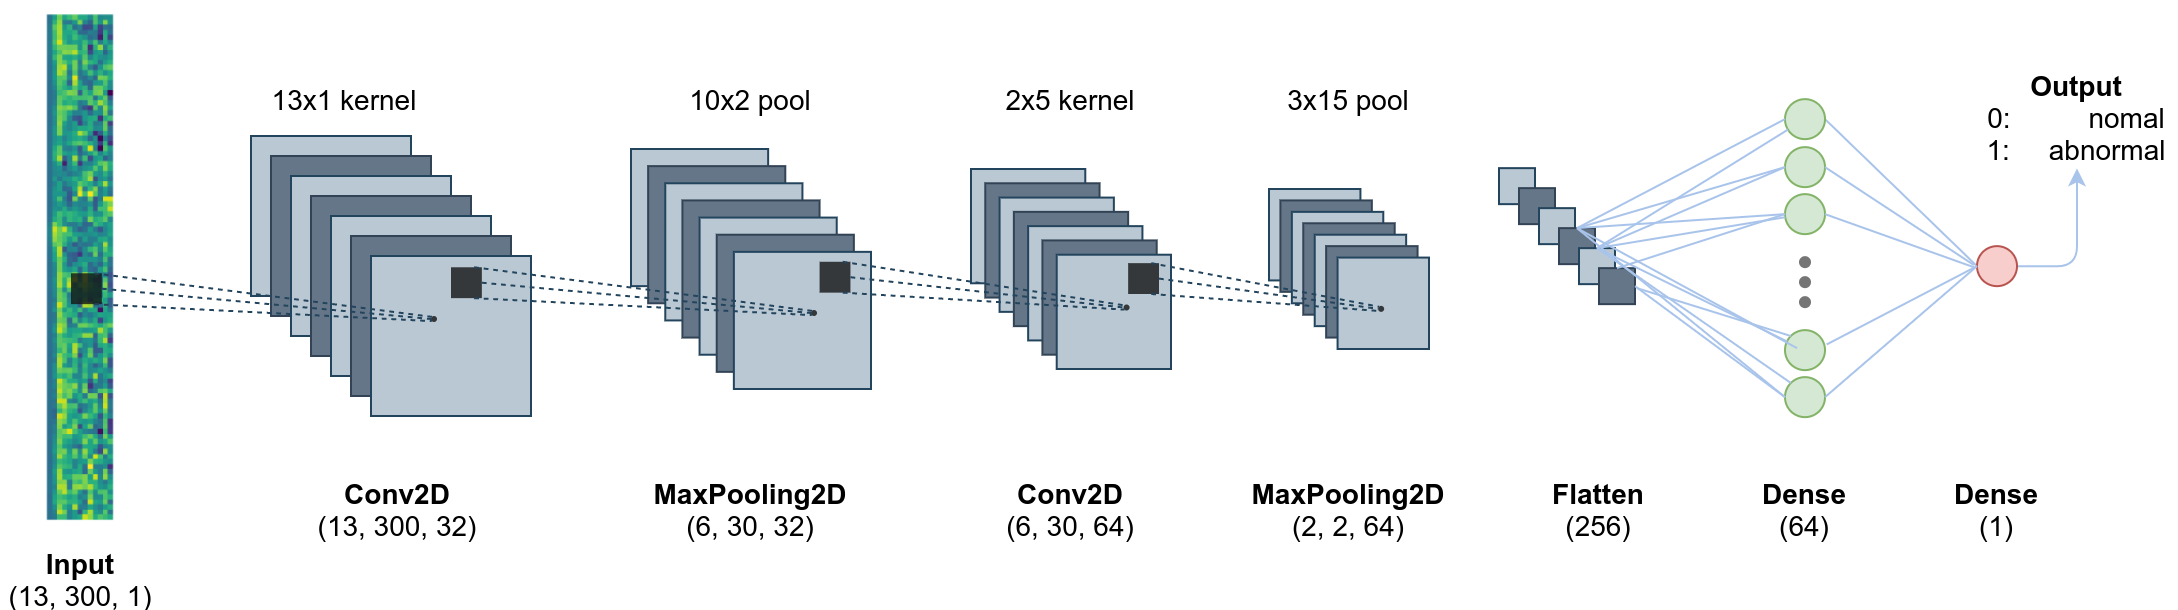
\includegraphics[width=\textwidth]{../images/cnn.png}
	\caption{Σχεδιάγραμμα της αρχιτεκτονικής του CNN δικτύου μας}
	\label{cnn}
\end{figure}


\subsection{Εκπαίδευση}

Για να εκπαιδεύσουμε τον δίκτυό μας χρησιμοποιήσαμε ένα σύνολο από 3240
φωνοκαρδιογραφήματα που παρείχε η Physionet \cite{physionet} στους
διαγωνιζόμενους. Από αυτά τα δείγματα χρησιμοποιήσαμε το 60\% για εκπαίδευση του
δικτύου και το 40\% για επαλήθευση της ακρίβειάς του. Στην συνέχεια εκπαιδεύσαμε
το δίκτυο για 50 εποχές με μέγεθος παρτίδας 32.

\end{document}
